\section{Forward-Mode Automatic Differentiation}
\frame{\tableofcontents[currentsection]}

\begin{frame}{Example Function and Expression Graph}
\[(x(t), y(t)) = (\cos(\omega t), \sin(\omega t))\]

\pause%
% Original expression graph
\begin{figure}[t]
\centering
\scalebox{0.9}{%

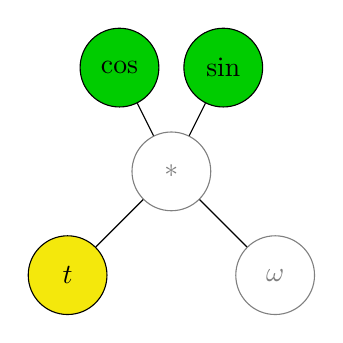
\begin{tikzpicture}[x=0.75pt,y=0.75pt,yscale=-0.5,xscale=0.5]

    \draw (200,350) node [align=center, minimum size=1cm, draw, circle, fill=black!5!yellow] (t)  {$t$};
    \draw (400,350) node [align=center, minimum size=1cm, draw, circle, color=gray] (omega)  {$\omega$};
    \draw (300,250) node [align=center, minimum size=1cm, draw, circle, color=gray] (mul) {$*$};
    \draw (250,150) node [align=center, minimum size=1cm, draw, circle, fill=black!20!green] (cos) {$\cos$};
    \draw (350,150) node [align=center, minimum size=1cm, draw, circle, fill=black!20!green] (sin) {$\sin$};
    \draw (t) -- (mul);
    \draw (omega) -- (mul);
    \draw (mul) -- (cos);
    \draw (mul) -- (sin);

\end{tikzpicture}
} % end scalebox

\end{figure}
\end{frame}

\begin{frame}{Forward AD}
\begin{itemize}
    \item Each node is represented by a \emph{dual number}, $(w, \frac{dw}{dx})$.
    \item Extend elementary functions to dual numbers.
    \item Unary $f$:
    \begin{align*}
        f( (w, \frac{dw}{dx}) ) := \paren{f(w), \frac{df}{dw} \frac{dw}{dx}}
    \end{align*}
    \item Binary $f$:
    {\small
    \begin{align*}
        f\paren{(w_1,\frac{dw_1}{dx}), (w_2, \frac{dw_2}{dx})}
        :=
        \paren{f(w_1,w_2), \frac{df}{dw_1} \frac{dw_1}{dx} + \frac{df}{dw_2}\frac{dw_1}{dx}}
    \end{align*}
    }
\end{itemize}
\end{frame}

\begin{frame}{Forward AD}
\begin{itemize}
    \item Example: 
    \begin{align*}
        \sin( (w, \frac{dw}{dx}) ) &= (\sin(w), \cos(w) \frac{dw}{dx})
        \\
        (w_1, \frac{dw_1}{dx}) \cdot (w_2, \frac{dw_2}{dx})
        &=
        (w_1 w_2, \frac{dw_1}{dx} w_2 + w_1 \frac{dw_2}{dx})
    \end{align*}
\end{itemize}    
\end{frame}

\begin{frame}{Forward AD Evaluation}
\begin{figure}[t]
\centering
\scalebox{0.9}{%

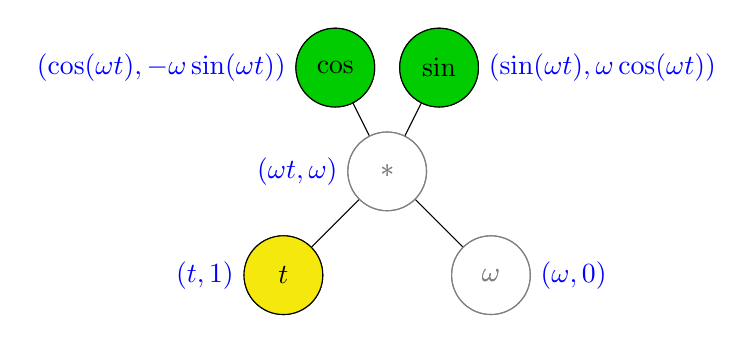
\begin{tikzpicture}[x=0.75pt,y=0.75pt,yscale=-0.5,xscale=0.5]

    \draw (200,350) node [align=center, minimum size=1cm, draw, circle, fill=black!5!yellow] (t)  {$t$};
    \draw (400,350) node [align=center, minimum size=1cm, draw, circle, color=gray] (omega)  {$\omega$};
    \draw (300,250) node [align=center, minimum size=1cm, draw, circle, color=gray] (mul) {$*$};
    \draw (250,150) node [align=center, minimum size=1cm, draw, circle, fill=black!20!green] (cos) {$\cos$};
    \draw (350,150) node [align=center, minimum size=1cm, draw, circle, fill=black!20!green] (sin) {$\sin$};
    \draw (t) -- (mul);
    \draw (omega) -- (mul);
    \draw (mul) -- (cos);
    \draw (mul) -- (sin);

    \pause%
    \draw (200,350) node [align=center, minimum size=1cm,
                          draw, circle, fill=black!5!yellow,
                          label={[blue]left:$(t,1)$}] (t) {$t$};
                          
    \pause%
    \draw (400,350) node [align=center, minimum size=1cm,
                          draw, circle, color=gray,
                          label={[blue]right:$(\omega,0)$}] (omega) {$\omega$};
                          
    \pause%
    \draw (300,250) node [align=center, minimum size=1cm,
                          draw, circle, color=gray,
                          label={[blue]left:$(\omega t, \omega)$}] (mul) {$*$};
                          
    \pause%
    \draw (250,150) node [align=center, minimum size=1cm,
                          draw, circle, fill=black!20!green,
                          label={[blue]left:$(\cos(\omega t), -\omega \sin(\omega t))$}] (cos) {$\cos$};
                          
    \pause%
    \draw (350,150) node [align=center, minimum size=1cm,
                          draw, circle, fill=black!20!green,
                          label={[blue]right:$(\sin(\omega t), \omega \cos(\omega t))$}] (sin) {$\sin$};

\end{tikzpicture}
} % end scalebox

\end{figure}
\end{frame}

\begin{frame}{Forward AD}
\begin{itemize}
    \item Easy to implement.
    \item Fast for $f:\R^n \to \R^m$ where $m \gg n$ ($O(n)$ sweeps of computation graph).
    \item Useful in physics applications when differentiating w.r.t. time.
    \item Example code (\code{fwd\_ad}).
\end{itemize}
\end{frame}